\documentclass{article}[11pt]
\setlength{\topmargin}{-2cm}
\setlength{\textheight}{24cm}
\setlength{\oddsidemargin}{10mm}
\setlength{\evensidemargin}{10mm}
\setlength{\textwidth}{15cm}
\setlength{\parskip}{3mm}
\setlength{\parindent}{0mm}

\usepackage{epsfig}
\usepackage{comment}
\usepackage{graphics}
\usepackage{graphicx}
\usepackage{hyperref}
\usepackage{times}
\usepackage[authoryear,round]{natbib}
\usepackage{subfigure}

\newcommand{\Rfunction}[1]{{\textsf{#1}}}
\newcommand{\Robject}[1]{{\texttt{#1}}}
\newcommand{\Rpackage}[1]{{\textit{#1}}}
\newcommand{\Rslot}[1]{\textsl{#1}}
\newcommand{\Rclass}[1]{\texttt{#1}}
\renewcommand{\baselinestretch}{1.5}

\begin{document}

\bibliographystyle{amsplain}

\author{Elizabeth Whalen\\Harvard School of Public Health}
\title{Generalizing the Model View Controller Paradigm}

\maketitle

\begin{abstract} 
  In this paper we consider a generalization of the model
  view controller (MVC) paradigm to allow for more flexible handling
  of submodels.  Instead of using a single MVC we develop a tree
  structure of related MVCs, where each MVC has a single parent, but a
  parent can spawn many different child MVCs.  Communication between
  parent and child MVCs allows for very flexible linking of the
  MVCs.  We provide an implementation of our work in the R package
  \Rpackage{MVCClass} available at \url{http://www.bioconductor.org}. 
\end{abstract}


\section{Introduction}\label{Sec:Intro}

%\subsection{Background}\label{Ssec:Backg}

%There are many ways to visualize multivariate data where more than
%two or three dimensions are needed to view the data.  Several of these ideas
%were discussed in previous work \cite{EW05}, so the focus in this paper
%is on one specific method of visualizing multivariate data that is
%particularly useful for exploratory data analysis; creating linked,
%interactive views of linked data sets.  

There are many ways to visualize multivariate data when more than
two or three dimensions are needed to view the data.  Many authors
\citep{intGrUnwin, DynGraphics, IEEEVisual, GGobi, DataDesk}
have suggested that linked, interactive views of the data
provide a valuable and important set of tools for comprehending such
data.  The model view controller (MVC) paradigm is now a standard
mechanism for implementing such systems.  The paradigm has proven very
effective and allows for clear separation of different components.
In this paper we consider an extension of the MVC paradigm to allow
for, what we believe to be, an easy expansion to linked data sets.

The sorts of problems we are interested in, are those where a user
might begin with a large data set, identify some interesting subset
and want to create interactive views of that subset.  In some cases the
natural data representation of the subset is in a form other than that
of the initial data set.  This leads to complications in the usual MVC
paradigm, where the data (i.e. the model) are often presumed to be in
a single, standard format.  We found that adding new views under such
conditions could be quite problematic and often led to very complex
code.  As we shall demonstrate, there are also issues that arise due to
mappings that are not one-to-one between elements on different views.
Hence we considered an approach that created new instances of
the \Robject{MVC} that were linked to the parent that spawned them.

In particular, our implementation consists of a hierarchy of \Robject{MVCs},
stored as a tree.  Each parent can have multiple children, but the
children have a single parent.  Communication between parent and
child is bidirectional, and a variety of different filters can be used
to control flow.  Thus, we can devise a number of purpose built \Rclass{MVC}
classes, each with a model appropriate to the specific data of
interest, that can be linked in a natural way.  Interacting with the view
in a child \Robject{MVC}, first sends a message to the child \Robject{MVC},
which will update all of its views, but the message will also propagate to the
parent \Robject{MVC} (and further up to the root).  The parent \Robject{MVC}
can choose whether to react to messages from its children -- all control being
in the hands of the users, should they want it.

\subsection*{A motivating example}
\label{sec:micro}

Our development of this model was driven primarily by an interest in
analyzing high throughput biological data.  Such data tend to be large
and very complex, and hence ideally suited to interactive
visualization.  In order to provide the reader with some idea of the
sorts of interactions we would like to support, we provide here a short
description of a type of experiment and some of the likely
interactions that would be of interest to a data analyst.

A gene expression experiment provides data on the expression of mRNA
abundance on thousands to tens of thousands of genes for some number
of samples.  Usually there are many fewer samples than genes.  There is
much that is known about the genes, such as what chromosome they are
located on and what sorts of activities they are engaged in, and in many
cases we want to restrict attention to a specific subset of genes, or
to alter the view so that rather than being gene centric it becomes
centered on some biological aspect, such as chromosome location.

One particularly rich data source is the Gene Ontology (GO), \cite{GO}
which provides three controlled vocabularies that are represented as
directed acyclic graphs, with a root node.  Terms typically have a
child-parent relationship, with the child terms being more specific
and the parent terms more general.  The root node represents the most
general term.  Genes are then annotated at specific nodes in these
graphs where the node is determined, by a domain expert, to describe a
property of the gene.  A gene is then also associated with all parents,
since if the specific term applies so must all more general ones.

There is often substantial interest in relating gene expression data
to such a graph based model, or to chromosomal locations, or to
activity in known biological pathways. Data mappings for this latter
aspect can be obtained from different sources such as \cite{KEGG}.
Further, users typically want to begin with a heatmap view. Then from
that derive a GO graph view, and additionally a chromosomal location
view. In order to interact with the GO graph, the primary unit is the
node in that graph (and sometimes one expects with the edges), while
for the heatmap view the basic element is generally the gene.  In Figures
\ref{Fig:heatmap} and \ref{Fig:GOgraph}, a heatmap view of gene expression
from Chronic Lymphocytic Leukemia (CLL) patients and the corresponding GO
graph are shown, respectively.  By interacting with the heatmap to color one
gene blue (shown as gene PDE8A on the heatmap), which causes the corresponding
GO nodes to be colored blue, one can easily see how this gene relates to the
GO terms.  Also by interacting with the node with an arrow next to it in
Figure \ref{Fig:GOgraph}, which represents the signal transducer activity GO
term, one can create a heatmap view that shows only the genes annotated at
that node, as shown in Figure \ref{Fig:heatmapsub}.  Notice how all genes
annotated at the signal transducer activity GO term have a blue label in
Figure \ref{Fig:heatmapsub}, which shows that this view was derived from a
blue colored node in Figure \ref{Fig:GOgraph}.  Compare the heatmaps in
Figures \ref{Fig:heatmapsub} and \ref{Fig:heatmap}.  The heatmap in Figure
\ref{Fig:heatmapsub} is just a subset of the heatmap in Figure
\ref{Fig:heatmap}, however in Figure \ref{Fig:heatmapsub} eleven genes have a
blue label and in Figure \ref{Fig:heatmap} only one gene has a blue label.
This difference in these heatmaps indicates that views are synchronized based
on the parent-child relationships.  Figure \ref{Fig:heatmap} is the parent of
Figure \ref{Fig:GOgraph}, which is the parent of Figure \ref{Fig:heatmapsub}.
Figures \ref{Fig:heatmap} and \ref{Fig:GOgraph} are synchronized, and Figures
\ref{Fig:GOgraph} and \ref{Fig:heatmapsub} are synchronized, but Figures
\ref{Fig:heatmap} and \ref{Fig:heatmapsub} are not synchronized by color
because they do not have a parent-child relationship: Figure \ref{Fig:heatmap}
is the grandparent of Figure \ref{Fig:heatmapsub}.

\begin{figure}[ht]
  \begin{center}
    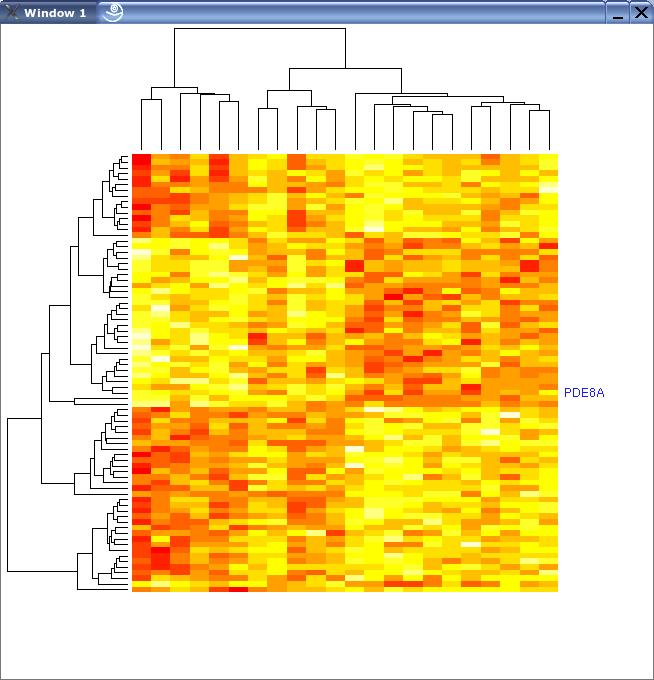
\includegraphics[height=5in, width=5in]{heatmap.jpg}
    \caption{ Heatmap view of gene expression from Chronic Lymphocytic
      Leukemia (CLL) patients. }
    \label{Fig:heatmap}
  \end{center}
\end{figure}

\begin{figure}[ht]
  \begin{center}
    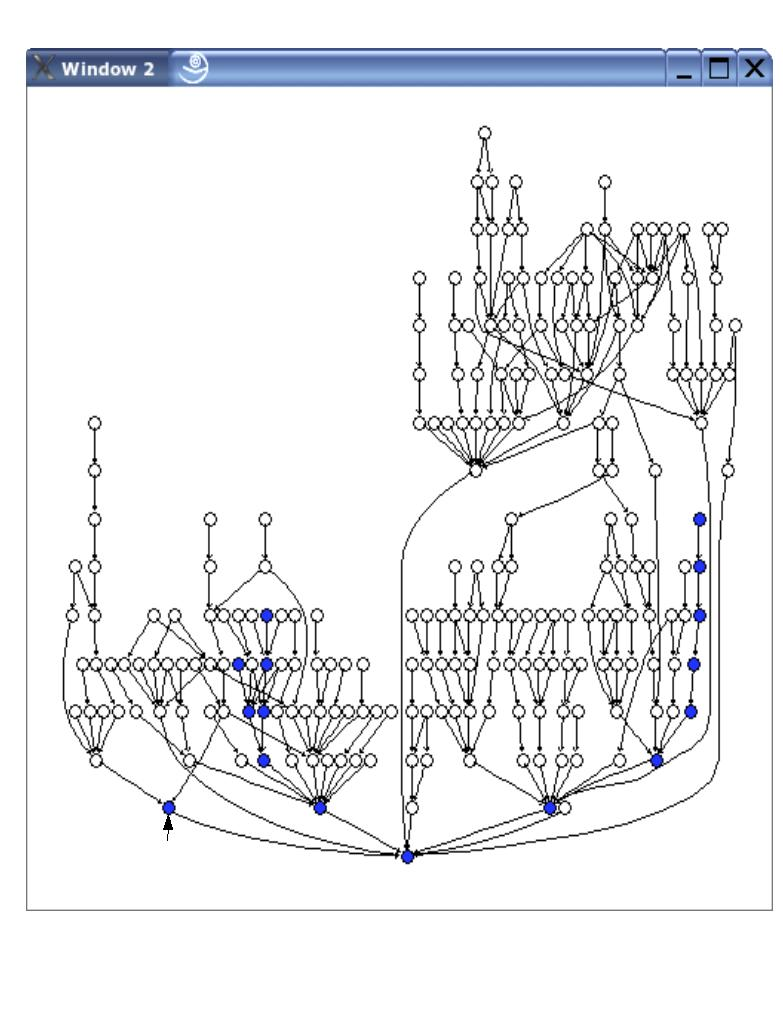
\includegraphics[height=4.3in, width=4.3in]{GOgraph2.jpg}
    \caption{ Gene Ontology (GO) graph that is associated with the genes
      displayed in the heatmap in Figure \ref{Fig:heatmap}.  Notice that one
      gene (PDE8A) is colored blue in the heatmap and all of the corresponding
      GO terms are colored blue in the graph.  The arrow next to one of the
      nodes indicates that this node was used to create the view shown in
      Figure \ref{Fig:heatmapsub}.  The node with the arrow next to it
      represents the signal transducer activity GO term. }
    \label{Fig:GOgraph}
  \end{center}
\end{figure}

\begin{figure}[ht]
  \begin{center}
    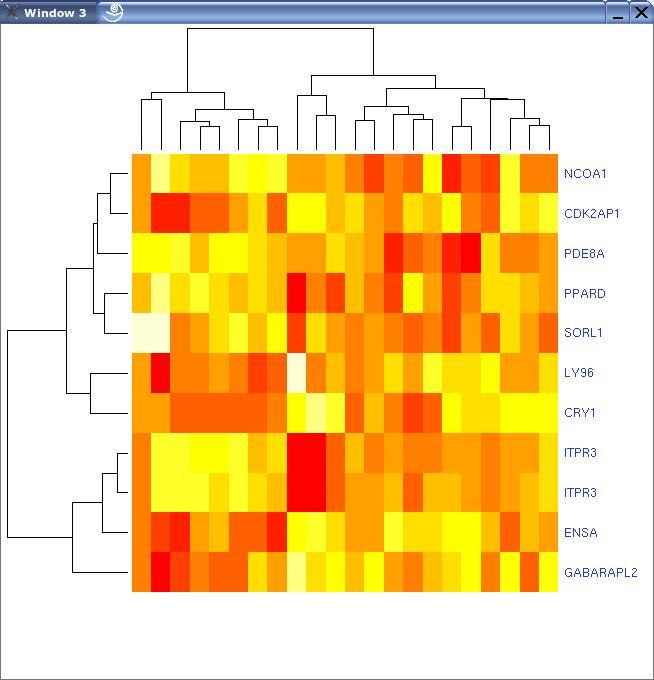
\includegraphics[height=5in, width=5in]{heatmapsub.jpg}
    \caption{ A heatmap view that shows only the genes that are annotated at
      the node in Figure \ref{Fig:GOgraph} that has an arrow next to it.  This
      node represents the GO term, signal transducer activity, and as shown in
      this heatmap, eleven genes are annotated at this node.  Notice that all
      the labels in this heatmap are colored blue, indicating that the parent
      node that was used to create this view was also colored blue.  
     }
    \label{Fig:heatmapsub}
  \end{center}
\end{figure}

\subsection*{Overview}
\label{Ssec:Over}

We found that constructing a single MVC that would encompass all
anticipated views was very cumbersome. It would also be inefficient
since a MVC model for the GO graph, or for a chromosome view would
also be of substantial interest, regardless of whether there was an
initial heatmap view or not. Thus, we looked for a solution that was
based more on component software constructed within an object oriented
programming environment.
%%FIXME: cite the JSS submission
We had several objectives, or design criteria. They were that the
software should be extensible in a high level language. We chose R as
the language for our implementation and wanted to allow users that
knew no other languages to be able to extend and enhance the
system.  Therefore, we built our software on top the \Rpackage{RGtk} package of
D. Temple Lang, since it provides such an interface. We also vastly
preferred Gtk+ over Tcl/Tk since its widgets are more sophisticated,
which we found results in a much shorter development time.

We wanted to provide a system that was usable and extensible by
relatively naive end users and hence have provided a graphical user
interface (GUI) which they can use to both carry out an analysis, but
also supports a variety of extensions, such as changing the actions
performed in response to events. We also wanted to support a more
sophisticated developer who might want to take our basic infrastructure
and create an interactive system, say for the interactive analysis of
time series data, using our design. Hence, all commands are
available both through the GUI and through command line functions.

\section{Methods}
\label{Sec:Methods}

First definitions of linked views, interactive views and linked data
sets are given in the following paragraphs.  Linked views mean that if a
component that represents data (such as a point on a plot or a row in a
spreadsheet) changes its appearance on one view, then the corresponding
component on a second view also changes its appearance.  For components on
different views to be corresponding, the data displayed in those components
must come from the same entity in a model.  As an example, suppose that the
model consists of the gene expression levels from four samples.  If the same
one hundred genes are studied in the four samples, then the model could be
represented as a matrix of four columns by one hundred rows with four columns
for the four samples and one hundred rows for the one hundred genes.  In this
model, the entities are the genes.  If two scatter plots are created as views
of this model, where the first plot displays sample one versus sample two and
the second plot displays sample three versus sample four, then the points on
each plot that referred to the same gene are corresponding components.  Linked
views, which have a long history in statistics, are now considered a standard
feature of interactive data visualization software \cite{GGobi}.  Linked views
have been implemented in several pieces of statistical software, such as
XLisp-Stat \cite{Lisp}, iPlots
\cite{iPlots}, and GGobi \cite{GGobiMan}.  Implementing linked views
is based on the model-view-controller (MVC) design \cite{DesignPatterns},
which is a widely used and well understood paradigm.  The MVC design is
discussed in more detail in Section \ref{Ssec:Design}.

Interactivity is an idea that is familiar from using an Internet browser.
Clicking on a hyperlink on a web page results in a new web page
opening.  Another example is clicking on the login button after entering a
user name and password to view one's email.  Interactivity means that there is
a response to some user action.  It is a powerful paradigm and allows users to
quickly navigate and explore complex documents or complex data sets.  As an
example, suppose that a user has two views: one view is a graph representing
the molecular function of genes and the other view is a heatmap of gene
expression data.  If the user clicks on a node that represents a particular
molecular function, then the response to this action could be to highlight all
genes in the heatmap view that correspond to this molecular function.  This
interactivity allows the user to quickly see if genes with the same molecular
function have similar expression levels. 

One particular model for creating interactive applications involves three
components: some user action or input, which is referred to as an event;
a response to that action, which is executed by a function that is called
a callback function; and a method that connects the event to the callback
function, which is referred to as the signal handler.  The events can
range from the user moving the cursor over a plot, to pressing a button on a
graphical user interface (GUI), to pressing certain keys.  Events are
interpreted based on which window has focus.  For example, in the XWindows
system, if a user types C on the keyboard and the window that has focus is a
text editor, then the letter C is printed on the text editor's screen.
Any other open windows that do not have focus do not respond to this event.
The callback function is a unique function because its signature is determined
by the event that the callback function is linked to.  The parameters passed
to the callback function may include information about the event, such as the
on screen location of the event, and information about the object that had
focus when the event occurred, such as a button on the GUI.  The signal
handler is the piece that must look to see if an event has occurred and then
when the event has occurred, the signal handler calls the appropriate callback
function. 

The strengths of this model of interactivity are that programmers can decide
which events to react to by deciding which signal handlers to implement,
programmers can change the response to an event by changing the callback
function that is linked to an event, and the system's event loop can continue
working on other things until a signal is emitted when an event occurs.  A
system's event loop controls how work is processed.  The event loop checks for
work to do and handles that work.  In the model of interactivity described
above when a signal handler is implemented by the programmer, this results in
the event loop periodically checking to see if an event has occurred.  Thus,
the event loop can perform other work and then check back to see if an event
has occurred.

These three pieces in this model of interactivity are ordered as follows:
an event occurs, the event causes a signal to be emitted that is caught by the
signal handler, and then the signal handler calls the callback function, which
results in the response to the user action.  A flowchart of these steps is
shown below in Figure \ref{Fig:Event}.  In the example of clicking on a
hyperlink mentioned above, the event is the user clicking on the
hyperlink and the callback function causes a new web page to open.
The signal handler, which is the method that connects the event to the
callback function, is handled by the system's event loop when a signal is
emitted. 

\begin{figure}[!h]
  \begin{center}    
    \scalebox{0.55}{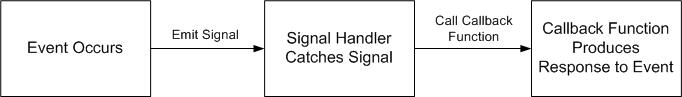
\includegraphics{Event.jpg}}
    \caption{ Flow chart of the response to an event. }
    \label{Fig:Event}
  \end{center}
\end{figure}

Linked data sets mean that the data have more than one conceptual grouping,
but there is a relationship between these different conceptual groupings.
Linked data sets are an idea that is familiar to users of relational
databases.  Data in a relational database are typically stored in many
linked tables with rows in different tables linked to each other through a
unique identifier called a key.  In this example, each table is
considered a data set and they are linked through the keys.  Another situation
where linked data occur is when there is experimental or study data that
are linked to meta-data.  An example of this situation is given in Section
\ref{Ssec:Limit} where the experimental data are microarray data, which looks
at gene expression levels, and the meta-data are a Gene Ontology graph that
gives the molecular functions of the genes studied in the microarray
experiment.  

Creating linked, interactive views of data is flexible for exploring
multivariate data because many different views can be created, such as
scatter plots, spreadsheets, and heatmaps, and these views are linked because
they are based on the same underlying data.  Thus, users can decide which
views best visually represent their data.  Also, since the views are
interactive, users can change the views while looking at them to make the
views more informative about the underlying structure in the data.  This
flexibility in linked, interactive views gives users a powerful tool for
visually exploring their data.  However, linked views can not solve all
problems.  Clearly, only a few linked views can be viewed simultaneously by
the user because only a certain number of views can be shown on a computer
screen.  Thus, there is a limit to the number of dimensions that can be
represented by linked views. 

Consider Figure \ref{Fig:firstMP}, which provides a cartoon
description of the steps that occur when a user interacts with a
view.  In the cartoon there are only two views, one of model A (note 
that once a data set is loaded in a MVC, we call it a model) and the
other of the linked model B.  When a user interacts with the scatter plot view
of model B, the response to this interaction is for model B to update itself
(this is indicated on the figure as a circled 1).  In Step 2, the scatter plot
view is told to update itself.  Next, in Step 3, because model B is linked
to model A, model B sends a message to model A.  In Step 4,
the information from model B is converted into information that
model A understands.  In Step 5, this information is received by
model A and model A updates itself.  Finally, in Step 6, model
A tells its view to update itself.  This example shows the components
and the communication between the components that are necessary to create
linked views of underlying linked data.  

In the design presented in this paper, the components consist of \Robject{MVC}
objects and communication within and between \Robject{MVC} objects is
performed by message objects.  This solution uses the power and simplicity of
the MVC design and expands it to the multiple data set problem.  Now we can
build on the original MVC design, which has been well tested, instead of
starting a new design from scratch.  The strength of this multiple linked MVC
design is that it uses MVC components, which can be individually created and
then linked.  Thus, these components are reusable.  These design decisions are
discussed further in Sections \ref{Sec:OneMVC} and \ref{Sec:MultMVC}. 

\begin{figure}[ht]
  \begin{center}
    \scalebox{0.55}{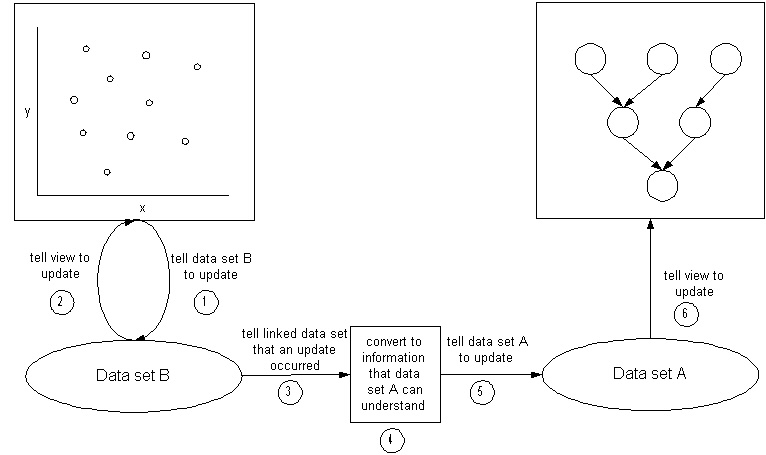
\includegraphics{firstMessagePassing.jpg}}
    \caption{ Linked views of linked models.  When a user interacts with
      the scatter plot, the first step, indicated by a circled 1,
      is to tell model B to update.  Then all views of model B must be
      updated.  Next any data that are linked to model B must be notified
      that model B changed.  This information from model B must be
      altered so that it can be understood by linked models, which is shown
      in the fourth step.  Finally, model A is notified that it should
      update in response to the change in model B and then all views of
      model A are updated. }
    \label{Fig:firstMP}
  \end{center}
\end{figure}

In Section \ref{Ssec:Design}, the design of linked, interactive views based on
the MVC paradigm is discussed.  However, the limitation with this design is
that it expects one data set, which limits the type of data we can visualize.
Thus, after discussing the limitations of
the MVC design in Section \ref{Ssec:Limit}, an extension of the MVC design is
discussed in Section \ref{Sec:Extend}.  This extension supports the creation of
linked \Robject{MVC} objects.  The design of individual \Robject{MVC} objects
is discussed in Section \ref{Sec:OneMVC} while the implementation of linked
\Robject{MVC} objects is discussed in Section \ref{Sec:MultMVC}.  The goals of
the software discussed in this paper are to create linked views of linked data
sets, to create interactive views where the response to an event can be
changed, and to create an extensible design that allows future users to make
additions. 

\subsection{Design and Implementation of Linked, Interactive Views}
\label{Ssec:Design} 

Focusing on linked, interactive views as a powerful visualization tool, the
next step is to determine how to design a software package that can implement
this method.  A popular design for creating linked views of data is the
MVC paradigm.  This design consists of three types of objects: the controller,
which defines what actions occur in response to user input; the view, which
consists of displays of the data; and the model, which manages the data.  This
paradigm is powerful because it decouples the views from the model.  Thus,
only one copy of the data need to be stored and then all views refer to this
data set.  With all views based on the same data, any changes to the data can
be propagated to all views, which creates linked views. 

To link the views to this one data set there is a subscribe/notify procedure
between the views and the model.  The views subscribe to a particular model
and the model must notify the views when a change occurs so that the views
are updated.  This design allows multiple views of the model that are
linked, but are not aware of each other, as shown in Figure \ref{Fig:ExMVC}.
Each view is responsible for visually representing some aspect of the model
and thus, it is not necessary for a view to be aware of other views.  By
keeping each view ignorant of other views, views can added and removed without
affecting each other. 

\begin{figure}[ht]
  \begin{center}
    \scalebox{0.5}{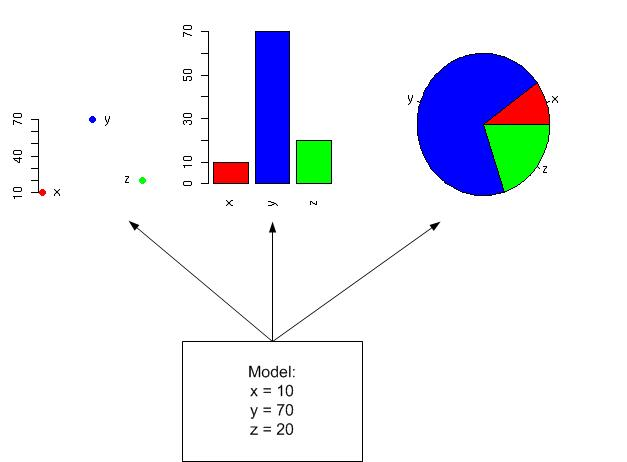
\includegraphics{ExMVC.jpg}}
    \caption{ A model with its views. }
    \label{Fig:ExMVC}
  \end{center}
\end{figure}

Notice that although the components (model, view, and controller) in the MVC
design are independent of one other, there needs to be communication
between them so that information can be shared.  Examples of this
communication between components include the model notifying views that the
data have changed, the controller asking the view which object on the plot the
user just interacted with, and the controller telling the model that the data
should change in response to user interaction with the view.  This message
passing between components in the MVC paradigm is discussed in detail in
Section \ref{Ssec:OneMess}.   

In \cite{EW05}, we discuss the creation of \textsf{R} software to fulfill
three goals: to create views that are linked, to create views that are
interactive, and to create a design that is extensible.  To implement the
overall goals of the design, two \textsf{R} packages, called
\Rpackage{MVCClass} and \Rpackage{iSPlot}, were created.  The
\Rpackage{MVCClass} package implements the class and generic function
definitions needed for the MVC design and the \Rpackage{iSPlot} package
creates the front end to let the user create linked, interactive views of
two-dimensional data, such as data frames and matrices, through a GUI or
through command line functions.  The reason for separating the software into
two packages was that it allowed the class definitions in the
\Rpackage{MVCClass} package to be used by any other \textsf{R} package that
wanted to create linked views.  

\subsection{Limitations of the MVC Design}
\label{Ssec:Limit}

The MVC design assumes that there is one data set, which is called the model,
that all views reference.  But problems arise when the data consist of more
than one conceptual grouping.  For example, consider data stored in a
relational database, where there are multiple tables of data and rows in
different tables are linked through a unique identifier called a key.
Although these tables of data could be combined into one large table, there
are several reasons not to do this.  Keeping the data in separate tables
reduces redundancy, particularly when the rows are related by a one-to-many or
a many-to-many relationship.  Also separate data tables generally lead to more
maintainable data.  By storing only one copy of each piece of information (in
a row in one table), it is easier to ensure that the data are correctly
updated when a change occurs.  All other tables that are connected with this
information can then just reference this row that has been updated. 

Consider Figure \ref{Fig:DBTab} shown below.  Here the database consists of
three tables, State, City and StateCity.  The State table has three columns,
State (the key), Life Expectancy, and Income.  The City table has three
columns, City (the key), Precipitation, and Temperature.  The StateCity table
has two columns, State and City.  This last table relates which cities are in
which states.  In this example, each city can be in only one state, but each
state can have more than one city so there is a one-to-many relationship
between states and cities.

\begin{figure}[ht]
  \begin{center}
    \scalebox{0.5}{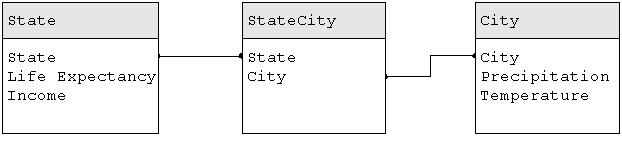
\includegraphics{newDatabaseTables.jpg}}
    \caption{ Example of relational database tables. }
    \label{Fig:DBTab}
  \end{center}
\end{figure}

Clearly, this information could be combined into one large table, called
CombinedStateCity, as shown in Figure \ref{Fig:OneDBTab}.  The
CombinedStateCity table has the following columns: State, Life
Expectancy, Income, City, Precipitation, and Temperature.  Now if a state's
life expectancy changes, all instances of this state need to change
in the new large table.  For example, if the state had the information for
three cities recorded, then the state has three rows in the
CombinedStateCity table and each row needs to change the value for the
state's life expectancy.  If instead only one record was kept per state, as
shown in Figure \ref{Fig:DBTab} above, then this process is less error
prone and requires less memory to store the data.  Another consideration in
combining data is that it may give the appearance of a relationship
between variables that does not exist.  For example, it may not make sense to
compare the Income data stored in the State table to the Precipitation data
stored in the City table.  Combining the data tables assumes that there is a
relationship between the variables in all of the tables.  This example shows
that there are advantages to storing the data in separate structures.

\begin{figure}[ht]
  \begin{center}
    \scalebox{0.5}{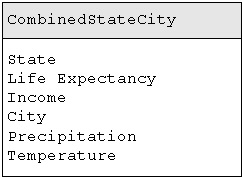
\includegraphics{newOneDatabaseTable.jpg}}
    \caption{ Example of a combined table. }
    \label{Fig:OneDBTab}
  \end{center}
\end{figure}

In a relational database all of the data are stored in tables, but consider the
situation where there are linked data that are of different data
structures.  For example, suppose that you have experimental microarray data,
which look at gene expression levels.  This experimental data can be
stored as a two dimensional data structure, such as a matrix, where rows are
genes and columns are samples.  Linked to this experimental data are meta-data
that give information about the genes studied in the microarray experiment.
For example, this meta-data may be terms from Gene Ontology, which form a
directed acyclic graph, describing the molecular functions carried out by
these genes.  The experimental data and the meta-data
are linked through the genes.  Each gene can have more than one molecular
function and each molecular function can have more than one gene annotated at
that function so there is a many-to-many relationship between the genes and
the molecular functions.  Though the data are linked, the
microarray data and the Gene Ontology data are different data structures.   

Now for the original MVC design, where one grouping of the data is expected,
it is not clear how to combine the experimental data and meta-data.  The
meta-data graph could be stored as a matrix, but a graph is a data structure
that can be well represented as an object with slots for nodes and edges,
especially if the graph is sparse.  As with relational database tables,
combining the data complicates data storage, alteration, and retrieval.  For
example, by combining the data, a structure may be forced on the data that may
not fit well, especially if the original data are instances of different
classes.  In contrast, keeping the data stored separately in their original
structures simplifies the processes of storing, updating, and accessing the
data.   

\section{Extending the MVC Design}
\label{Sec:Extend}

As discussed in Section \ref{Sec:Intro}, the MVC design typically uses a single
conceptual unit, such as a data frame or a matrix, for the model.  And
we believe that such an approach is a good one.  MVCs should be
specialized to certain types of data, as this allows them to provide
better and more natural interactions.  However, we additionally argue
that there is great benefit to considering linking these different
MVCs when the underlying data themselves are derived from the same source.
We believe that there will often be a hierarchical relationship
between the models and the MVCs that contain them.  We have found
that allowing the user to create new MVCs based on a current MVC is an
important and useful paradigm.

Each \Robject{MVC} is a coherent object and the interactions between
\Robject{MVCs} are encapsulated in a set of messages.  We use one
\Robject{MVC} object to handle each model.  Thus, within a
\Robject{MVC} object, one can create linked views of that particular
model, using the standard MVC design.  Between \Robject{MVC}
objects we propose a second messaging system that allows messages to
be sent between linked models.

%In Section
%\ref{Ssec:Limit} we provided several examples where it is advantageous to link
%multiple data sets.  These examples included linked tables in relational
%databases and experimental data linked to meta-data.  Being able to visualize
%variables simultaneously from different data sets that are linked is useful
%for exploring relationships between these variables.  We next describe how
%the MVC design can be revised and extended to accommodate multiple data sets. 

%\subsection{One Large Data Set}\label{Ssec:OneDS}
%
%One possibility for dealing with multiple data sets within the MVC design is
%to combine the multiple data sets into one large data set.  With this new
%combined data, the original MVC design can be used to create linked views.
%
%Unfortunately, as discussed in Section \ref{Ssec:Limit}, combining
%multiple data sets into one large data set can be problematic.  Even if the
%multiple data sets have the same data structure, combining the data sets often
%results in redundant data and makes updating and representing the
%data more complicated.  In the situation where the data sets do not have the
%same structure, it may be necessary to define a new class to appropriately
%represent the combined data.  Also, combining the data into one data structure
%may give the appearance that some variables have a relationship that does not
%exist.  Just because two data sets are linked does not necessarily mean that
%there is a meaningful relationship between their data.  Thus, another way
%of linking views based on multiple data sets needs to be designed. 

%\subsection{Multiple MVC Objects}\label{Ssec:MMVC}
 

\small
\begin{tabular}[t]{ | l | r | r | }
  \hline
  State & Life Expectancy & Income \\ \hline
  Pennsylvania & 70.43 & 4449 \\ \hline
  California & 71.71 & 5114 \\ \hline
  Minnesota & 72.96 & 4675 \\ \hline
\end{tabular}
\hspace{10pt}
\begin{tabular}[t]{ | l | r | r | }
  \hline
  City & Precipitation & Temperature \\ \hline
  Philadelphia & 39.9 & 39 \\ \hline
  Pittsburgh & 36.2 & 37 \\ \hline
  Los Angeles & 14.0 & 68 \\ \hline
  San Francisco & 20.7 & 56 \\ \hline
  Sacramento & 17.2 & 55 \\ \hline
  Duluth & 30.2 & 18 \\ \hline
  Minneapolis St. Paul & 25.9 & 22 \\ \hline
\end{tabular}

\begin{table}[h]
  \begin{center}
    \begin{tabular}{ | r | r | }
      \hline
      State & City \\ \hline
      Pennsylvania & Philadelphia \\ \hline
      Pennsylvania & Pittsburgh \\ \hline
      California & Los Angeles \\ \hline
      California & San Francisco \\ \hline
      California & Sacramento \\ \hline
      Minnesota & Duluth \\ \hline
      Minnesota & Minneapolis St. Paul \\ \hline
    \end{tabular}
    \caption{State and city values.}\label{Tab:CityState}
  \end{center}
\end{table}

\normalsize
As an example, suppose that one has two models: one with information at the
state level and one with information at the city level.  These tables are
shown in Table \ref{Tab:CityState}.  The State data include Life Expectancy
(in years from 1970) and Income (per capita from 1974) data
while the City data include Precipitation (in inches from 1975) and Average
High Temperature in January (in Fahrenheit from 2005)
data.  These two models are linked by the StateCity table that links cities
with the states they reside in.  Now for these two models there are
two \Robject{MVC} objects.  One \Robject{MVC} object for the State data and
its views and one \Robject{MVC} object for the City data and its views. 

\begin{figure}[ht]
  \begin{center}
    \scalebox{0.7}{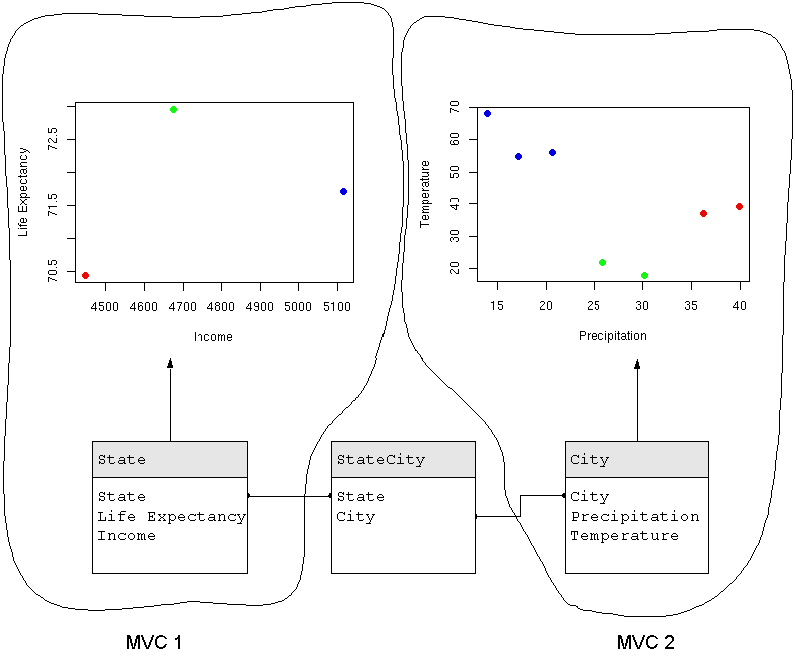
\includegraphics{MultipleMVC.jpg}}
    \caption{ Example of two \Robject{MVC} objects.  These two \Robject{MVC}
      objects are linked by the StateCity table and the color of the points
    indicates the linking between the data.  The points referring to the state
    of Pennsylvania are red, the points referring to the state of California
    are blue, and the points referring to Minnesota are green. }
    \label{Fig:MultMVC}
  \end{center}
\end{figure}

Figure \ref{Fig:MultMVC} shows one view for the State data and one view
for the City data.  You can see how the State and City data are linked based
on the coloring of the points in the plots.  The points referring to the state
of Pennsylvania are red, the points referring to California are blue, and the
points referring to Minnesota are green.  Even though there are two
\Robject{MVC} objects here, with one \Robject{MVC} object for each model,
it is still clear that the views are linked through the models and that is
shown in this example through the coloring.

Not only does this solution use the power and simplicity of the MVC design, but
this multiple MVC design is structured to fit the linking seen in the multiple
data sets.  Clearly, the design should be built around the problem and
multiple \Robject{MVC} objects with messaging between the \Robject{MVC}
objects fits the problem of creating linked views of multiple linked data
sets.  In designing an appropriate messaging system between \Robject{MVC}
objects, consideration is given to what information should pass between
\Robject{MVC} objects and to how messages propagate between \Robject{MVC}
objects.  As for the relationship between the \Robject{MVC} objects, it should
reflect the relationship between the data sets. 

Although two examples of linked data sets have been discussed thus far,
this paper focuses on experimental data that are linked to meta-data, as
the data we are most interested in visualizing.  In this situation, the
experimental data can be thought of as determining what meta-data are studied.
In the example of microarray experiment data linked to Gene Ontology
meta-data, only Gene Ontology data that refer to genes in the microarray
experiment are included in the meta-data.  Thus, there is a hierarchical
relationship between these data sets and the \Robject{MVC} objects that
contain them, where one \Robject{MVC} object creates another \Robject{MVC}
object.  The original \Robject{MVC} object is the parent \Robject{MVC} and the
new \Robject{MVC} object that is created from the parent \Robject{MVC} is the
child \Robject{MVC}.  These decisions are discussed in the following sections
as the design for multiple \Robject{MVC} objects is explained. 

\section{Design Details of One MVC Object}
\label{Sec:OneMVC}

\subsection{Implementation Details}
\label{SSec:OneOver}

Implementing linked, interactive views of linked data sets is done using an
object-oriented programming design for extensibility.  The \Rpackage{MVCClass}
package implements the design of the MVC classes and generic functions.  The
\Rpackage{MVCClass} package defines the individual model, view, and controller
classes as well as the \Rclass{MVC} class that binds the individual model,
view, and controller classes together into one unit.  The \Rpackage{MVCClass}
package also defines the message classes that allow the components to
communicate with each other.  Thus, the \Rpackage{MVCClass} package contains
the classes necessary for creating linked views.  Also, the
\Rpackage{BioMVCClass} package creates new model and view classes that extend
the classes available in the \Rpackage{MVCClass} package.  The goal of placing
these class and generic function definitions in other packages is that they are
available for other \textsf{R} packages that implement linked views of data,
such as the \Rpackage{iSPlot} and the \Rpackage{iSNetwork} packages.  

With the class definitions created in the \Rpackage{MVCClass} and the
\Rpackage{BioMVCClass} packages, the
\Rpackage{iSNetwork} package can decide which classes
to use based on the overall goals of the combined software.  The
\Rpackage{iSNetwork} package also determines how instances of these classes
behave because the methods for the classes are defined in the
\Rpackage{iSNetwork} package.  In addition to implementing the behavior of
objects, the \Rpackage{iSNetwork} package also creates a graphical user
interface (GUI) so that users can load data, create views, and interact with
the views through menus on the user interface.  As an alternative to the GUI,
users also have access to the same functionality through command line
functions.  

To create the GUI, \Rpackage{iSNetwork} uses the R packages,
\Rpackage{RGtk} and \Rpackage{gtkDevice}.  \Rpackage{RGtk} is an \textsf{R}
package that allows one to interact with Gtk+ functions from the \textsf{R}
interface.  Gtk+ is an open-source window toolkit \cite{Gtk} for creating user
interfaces.  The \Rpackage{gtkDevice} package creates a Gtk+ device by turning
a Gtk+ drawing area into a device that acts like an \textsf{R} device, but
still responds to events so that the view can be interactive.  For more
information about these packages, see \cite{EW05}.  

The next sections explain the class definitions and the methods that
pertain to a single \Robject{MVC} object.  Thus, the model classes,
the view classes, the controller, the \Rclass{MVC} class
(which binds the model, view and controller classes
together), and the message classes that pass information between the
three components in one \Robject{MVC} object are discussed in the following
sections.  All of the class definitions are implemented in the
\Rpackage{MVCClass} and \Rpackage{BioMVCClass} packages and all of the methods
are defined in the \Rpackage{iSNetwork} package.  Message class definitions
that pertain to communication between the \Robject{MVC} objects are discussed
in Section \ref{Sec:MultMVC}. 

\subsection{Model}
\label{Ssec:OneModel}

In the MVC design, the model component is the place where data are stored and
updated.  Thus, the model is a storage location that can perform certain
operations.  Information can be sent to the model to add, update, and remove
data and the model can send out messages that changes have occurred to the
data that the model stores.  Thus, the object model for the model
classes represents both the slots that are needed to store data and the
methods that are needed to perform the operations of the model. 

Figure \ref{Fig:Model} shows the inheritance structure for the model
classes.  Here the virtual class, \Rclass{gModel}, has the slots
\Rslot{modelData}, \Rslot{linkData}, \Rslot{virtualData}, \Rslot{modelName},
and \Rslot{modelVar}.  These five slots are common information that all models
need to store.  The \Rslot{modelData} slot is the data set for this model, the
\Rslot{linkData} slot is a list of two functions, \Rfunction{toParent} and
\Rfunction{fromParent}, which let this model send information to its parent
model and receive information from its parent model, respectively (see
Sections \ref{Ssec:OneMVC} and \ref{Ssec:MultLink} for more information on how
parent and child models are linked), the \Rslot{virtualData} slot is data
pertaining to the views that needs to be stored with the model so that it can
be shown in all views of this model, the \Rslot{modelName} slot is the
name of the model, and \Rslot{modelVar} is a list of any model variables,
which are extra data that are stored with the model, such as test statistics
calculated from the model data.  

\begin{figure}[ht]
  \begin{center}
    \scalebox{0.7}{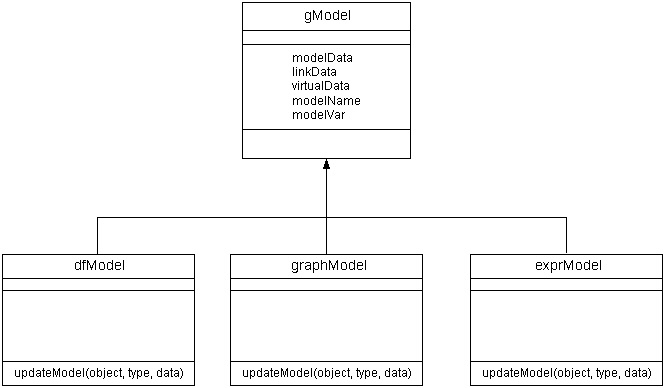
\includegraphics{ModelClass.jpg}}
    \caption{ Inheritance for model classes. }
    \label{Fig:Model}
  \end{center}
\end{figure}

We encapsulate the particular data model in the class definition, which allows
for efficient dispatch, and accessor functions that are appropriate for the
underlying implementation.  The specific model classes used in the
\Rpackage{iSNetwork} package to represent data are \Rclass{dfModel},
\Rclass{graphModel}, and \Rclass{exprModel}.  The \Rclass{dfModel} class
represents a model where the \Rslot{modelData} slot has class data frame (or
matrix), the \Rclass{graphModel} class represents a model where the
\Rslot{modelData} slot has class graph, and the \Rclass{exprModel} class
represents a model where the \Rslot{modelData} slot has class exprSet, a class
used to represent gene expression data \cite{BioC}.

As mentioned previously, the model classes must also perform certain
operations and these operations are reflected in the methods that are defined
for the classes.  All three model classes have an \Rfunction{updateModel}
method that is defined in the \Rpackage{iSNetwork} package.  This method is
called whenever the data need to be updated in response to a user interacting
with a view.  Thus, the \Rfunction{updateModel} method is actually updating the
\Rslot{virtualData} slot because it is this slot in the model classes
that ensures that all views are appropriately visually linked.  

Although only three model classes are currently implemented, future
users are welcome to make additions to the model classes for new data
structures they want to represent.  For example, a user may want to add a new
model class called \Rclass{tsModel} to represent time series data.
To make this addition, the user extends the \Rclass{gModel} class in his or
her own package. 

The model classes must also notify views when the data have changed
so that the views can be updated.  The communication between a model and its
views are discussed in Section \ref{Ssec:OneMess}. 

\subsection{Views}
\label{Ssec:OneViews}

The view classes represent the visual depictions, or renderings, of
the model.  There are some data that are required by all views, and all views
must respond to a certain subset of events so we have implemented the view
classes by first creating a single, virtual class which the specialized
views extend.  As with our model classes, this allows us to define
methods and data storage once, for the virtual class, and only extend
it for views that specifically require additional data storage, or
specialized handling.  The object model for the view classes is shown
in Figure \ref{Fig:View}.

\begin{figure}[ht]
  \begin{center}
    \scalebox{0.7}{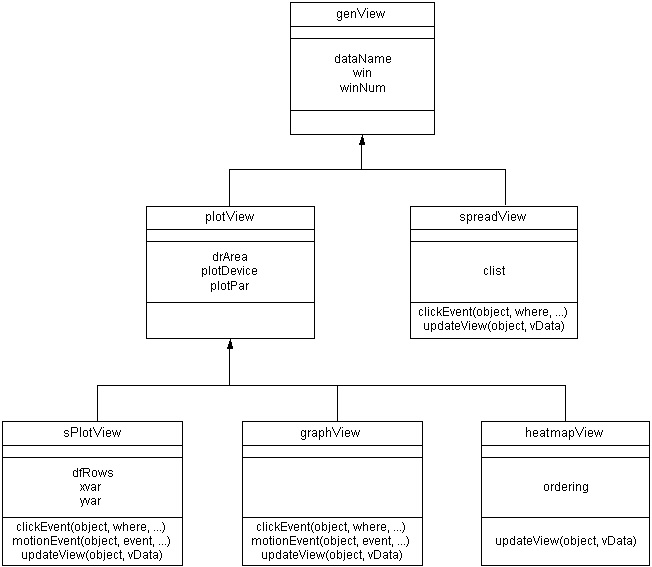
\includegraphics{newViewClass.jpg}}
    \caption{ Inheritance for view classes. }
    \label{Fig:View}
  \end{center}
\end{figure}

The \Rclass{genView} class has three slots, \Rslot{dataName}, \Rslot{win},
and \Rslot{winNum}.  \Rslot{dataName} is the name of the model that the view
displays, \Rslot{win} is the Gtk+ window object that holds the view, and
\Rslot{winNum} is the number of the window so that the window can be
identified in the Window menu on the GUI (see Section \ref{Ssec:OneCont}).
All views need to know these three pieces of information so
\Rclass{genView} binds the view classes together. 

As for specific view classes, the \Rclass{spreadView} class
represents a spreadsheet view of the data.  This view only makes sense for
models that are a two dimensional data structure, such as a matrix or a data
frame.  The information needed for this view is stored in the slot,
\Rslot{clist}, which is the Gtk+ spreadsheet object.

When creating a plot of a data set, there is a general class, called
\Rclass{plotView}, that has the slots, \Rslot{plotDevice}, \Rslot{plotPar},
and \Rslot{drArea}, which store the device number of the plot, the plotting
parameters, and the Gtk+ drawing area object, respectively.  This class is a
virtual class as it represents a general plot.  The instantiable plot classes
are the specific plot classes, \Rclass{sPlotView}, \Rclass{graphView}, and
\Rclass{heatmapView}, which inherit from the \Rclass{plotView} class.  

The \Rclass{sPlotView} class represents a scatter plot view and it has the
extra slots, \Rslot{dfRows}, \Rslot{xvar}, and \Rslot{yvar}, where
\Rslot{dfRows} are the row names from the model that are shown in the plot,
\Rslot{xvar} is the variable name from the model that is shown as the x
variable in the plot, and \Rslot{yvar} is the variable name from the model
that is shown as the y variable in the plot.  The \Rclass{graphView} class
represents a graph plot view and it contains the slot, \Rslot{grLayout}, which
holds a \Robject{Ragraph} object that represents the layout of the graph plot.
The \Rclass{heatmapView} represents a heatmap view of the data and it contains
the slots, \Rslot{ordering} and \Rslot{rNames}, where \Rslot{ordering} is a
list that is returned from the \Rfunction{heatmap} function to give
information about the ordering in the row and column dendrograms and
\Rslot{rNames} are the row names that were used to create the heatmap in case
a subset of the data was used to create the view.  Note that some of these
views are only applicable for certain model types.  For example, the
\Rclass{graphView} class only makes sense for a view of a graph object,
which is stored in the \Rclass{graphModel} class. 

Since all views are expected to be interactive they have methods that
correspond to the different supported user interactions.  The events
we are most interested in responding to include key press events,
where a certain configuration of keys are pressed; button click
events, where one of the mouse buttons is clicked over the view; and
mouse movement events, where the cursor moves over the view.  When an
event occurs it creates a signal, that is caught by the signal
handler.  The signal handler then calls the callback function and it
is in the callback function that the corresponding method is called.
For example, when the user clicks the mouse button and the cursor is
over a scatter plot view, it is the scatter plot's
\Rfunction{clickEvent} method that is invoked.  Then within the
\Rfunction{clickEvent} method, the \Rfunction{identifyView} method is called
to convert the pixel coordinates into an object in the plot.

As can be seen in Figure \ref{Fig:View}, \Robject{sPlotView},
\Robject{graphView}, \Robject{heatmapView}, and \Robject{spreadView} all have
a \Rfunction{clickEvent} method, which is called when the button click event
occurs or in the case of \Robject{spreadView} when a row is selected on the
spreadsheet. Currently, only \Robject{sPlotView} and \Robject{graphView} have
\Rfunction{motionEvent} methods, which is called when the cursor moves over
the view.  The \Rfunction{clickEvent} and \Rfunction{motionEvent} methods call
the \Rfunction{identifyView} method to determine which object on the view was
under the cursor.

As with the model classes, the view classes need an update
method and thus, all views have an \Rfunction{updateView} method that is
defined in the \Rpackage{iSNetwork} package.  This method must take the
information that a model has just been updated and appropriately update the
view to reflect that change.  Each method depends on how the view
represents the data so for a \Robject{spreadView} object the
\Rfunction{updateView} method may select or unselect a row on the spreadsheet
while for a \Robject{sPlotView} object the \Rfunction{updateView} method may
change the appearance of a point on the plot.  

Note that when updating a view in \textsf{R} we do not have access to objects
on a view.  Thus, a point on a plot is not an object that allows us to update
its attributes and then have that point redrawn to reflect its new attributes.
Instead in \textsf{R} we must currently draw over a portion of the view to
update the view.  However, if the method of creating \textsf{R} plots changed,
the \Rfunction{updateView} methods could be modified. 

The inheritance structure of the view classes is intended to be
extensible.  For instance, if users wanted to add a new plot view, say a
density plot, they could create a new view class that inherits from
\Rclass{plotView}, called \Rclass{dPlotView}.  This new class,
\Rclass{dPlotView}, has slots named \Rslot{dfRows} and \Rslot{col} to store
which rows and which column, respectively, were used to calculate the density
shown in the view.

\subsection{Controller}
\label{Ssec:OneCont}

The controller performs two tasks: the first task is to maintain state,
such as what response will occur for a particular user interaction, 
and the second task is to control message passing.  Messages, which are
discussed in Sections \ref{Ssec:OneMess} and \ref{Ssec:MultLink}, are
responsible for creating new components, such as models and views, and for
passing information between components, such as a view asking a model for
information.  The controller determines when these messages are created and
ensures that they are sent to the proper recipient.

For the first task, which is implemented in the \Rpackage{MVCClass}
package, the controller is implemented as an environment that is stored in the
\Rslot{controller} slot of a \Robject{MVC} instance, which is discussed in
more detail in Section \ref{Ssec:OneMVC}.  Although other options exist for
storing data, such as a list or a database, an environment is nice because in
\textsf{R} an environment is not copied each time a value within the
environment changes.  

For the second task, the controller gives the user restricted access
to the state information through an application program interface
(API) and thereby lets the user change the response to different events. 
In our implementation users can interact either through a GUI
or through command line functions.  Through the API the user can load
data, create views, set the response to user interaction with a view,
quit the program and perform other functions.  On the GUI, which is shown in
Figure \ref{Fig:ContWin} and is called the control window, users can decide
which action is taken next by interacting with one of the menus.  If the user
would rather not use the GUI, there are command line functions that
provide access to the same functionality that is available through the
GUI.  

\begin{figure}[ht]
  \begin{center}
    \scalebox{0.35}{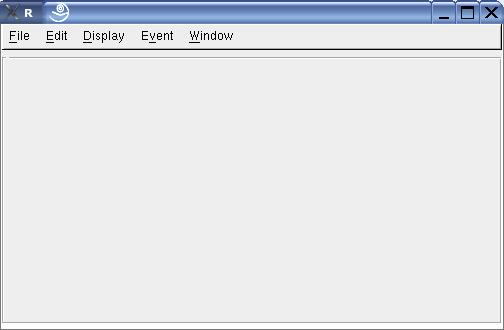
\includegraphics{ControlWindow.jpg}}
    \caption{ The control window. }
    \label{Fig:ContWin}
  \end{center}
\end{figure}

As shown in Figure \ref{Fig:ContWin}, the menus on the control window are
\texttt{File}, \texttt{Edit}, \texttt{Display}, \texttt{Event}, and
\texttt{Window}.  These menus always appear on the control window, but the
menu items under each menu change depending on the type of model that is
active.  Because the goal is to have multiple linked \Robject{MVC} objects,
more than one \Robject{MVC} object is loaded and thus, more than one model.
However, the control window menus and the command line functions only perform
operations on one \Robject{MVC} object at a time.  Thus, in the
\Rpackage{iSNetwork} package there is the concept of the \textit{active}
\Robject{MVC} object, where the \textit{active} \Robject{MVC} object (and
thus, the active model) means that operations performed through the control
window menus or through the command line functions affect that \Robject{MVC}
object.  For example, the \texttt{Display} menu allows users to create views
of the active model, but only certain views are appropriate for a type of
model, as mentioned in Section \ref{Ssec:OneViews}.  If the active model was a
data frame model (\Rclass{dfModel}), then the views that the user could create
are a scatter plot (\Rclass{sPlotView}) and a spreadsheet
(\Rclass{spreadView}), but a graph plot (\Rclass{graphView}) does not make
sense.  Thus, when the model in the \textit{active} \Robject{MVC} is of class
\Rclass{dfModel}, then the \texttt{Display} menu has menu items to create a
scatter plot and a spreadsheet.  Also, if the \textit{active} \Robject{MVC} is
of class \Rclass{dfModel}, then the command line functions only let the user
create a scatter plot and a spreadsheet view of the active model.

Because one of our goals is to create a software package that is
flexible and extensible, users and developers can add menus and menu items 
to the control window through the command line to access new
functionality that they have created.  As an example if a future
programmer wants to add a new type of view, such as a histogram, then
a new menu item for that view could be added to the \texttt{Display}
menu.  When adding to the API, command line functions should be created as
well as menu items to access the new functionality.

\subsubsection{Linking Events to Functions}
\label{Ssec:OneEvent}

Linking callback functions to events, such as a button click, a mouse movement
or a key press event, is what allows users to have an interactive
environment.  When an event occurs, the callback function linked to the event
determines the response to that event.  To create a flexible environment
it is nice to be able to change the response, which is determined by the
callback function, to an event.  For example, when a left button press event
occurs, a user may sometimes want a point to be colored and at other times she
may want a point to be hidden.  

To allow this flexibility in the response to an event, a class called
\Rclass{gEventFun} was created.  The \Rclass{gEventFun} class stores all of
the information needed to create a particular response to an event.
Clearly, the response to an event can be performed by a single function,
which is called the callback function, as discussed in Section
\ref{Sec:Intro}.  However, different responses to an event may require
functions with different signatures, where a function signature is the
combination of the function name along with its parameters.  Using the example
in the previous paragraph, a callback function that colored a point needs two
parameters, the new color to use and the point to color, while a callback
function that hid a point needs just one parameter, the point to hide.  Since
the intention is to be able to interchange the responses to an event, the
signatures of different callback functions should be the same.  These design
decisions determined the slots in the \Rclass{gEventFun} class and are
discussed more fully in the following paragraphs. 

As shown in Figure \ref{Fig:EventFun}, the slots in the \Rclass{gEventFun}
class are \Rslot{callFun}, \Rslot{shortName}, and \Rslot{preprocessFun}.  The
\Rslot{callFun} slot is the callback function, the \Rslot{shortName} slot is a
short description of the function that identifies the callback function, and
the \Rslot{preprocessFun} slot is a list of all preprocessing
functions that must be called before the callback function.

\begin{figure}[ht]
  \begin{center}
    \scalebox{0.6}{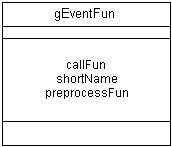
\includegraphics{EventClass.jpg}}
    \caption{ The gEventFun class. }
    \label{Fig:EventFun}
  \end{center}
\end{figure}

Since the intention is to be able to interchange the responses to an event,
the signatures of different callback functions should be the same.
In our design a callback function takes only one parameter. 
The class of that parameter depends on the type of model represented by the
\Robject{MVC}.  For example, for a graph model, the parameter corresponds to
the name of a node in the graph, while for a data frame model, the parameter
represents a case.  We expect a one-to-one relationship between the elements
on a view and the elements in the model.  Continuing the previous example,
each point on a scatter plot represents one case in the data frame model and
each node in the graph plot represents one node in the graph model.  Clearly
it is possible for two points in a scatter plot to overlap if they have the
same x axis and y axis values, but they are still considered two points
representing two cases in the model.

Any other information a callback function may need is set using the
preprocessing functions, which are automatically called once by the controller
when the callback function is linked to the event.  The preprocessing
functions take no parameters.  The purpose of the preprocessing functions is
to set variables that the callback function needs.  Thus, not all callback
functions need preprocessing functions.  If the callback
function sets the color of a node in a graph, then a preprocessing
function is needed to determine what color is used.  So in this
example, the preprocessing function opens a color browser to allow the
user to choose the new color.

Users can link actions to events either through the GUI or via
command line functions.  The controller environment for each \Robject{MVC}
object stores a list, for each event, of appropriate callback functions that
can be linked to that event and it also stores which callback function is
currently linked to the event.  When a developer creates a new callback
function, the developer can decide which events the callback function can
potentially be linked to.  For example, the developer may only want the color
a point callback function to be available for a button click event and not a
mouse over event.

\subsection{MVC}
\label{Ssec:OneMVC}
 
The \Rclass{MVC} class binds the model, view, and
controller objects into one object.  Thus, whenever a new data set
is loaded, a \Robject{MVC} object is created.  A \Robject{MVC} object can have
one model and each model must be in one \Robject{MVC}
object so there is a one-to-one relationship between the \Robject{MVC} and
model objects.  Because of this relationship, the \Robject{MVC}
object and the model object are identified by the same name, which
is stored in the \Rslot{modelName} slot of the model object.  When
loading a new model, the name of the model is checked to
ensure that it is unique.

As shown in Figure \ref{Fig:MVCClass}, there is a virtual class, \Rclass{MVC},
that binds the MVC inheritance structure together.  The virtual class,
\Rclass{MVC}, has three slots, which are \Rslot{model}, \Rslot{viewList}, and
\Rslot{controller}.  The \Rslot{model} slot stores the model object, the
\Rslot{viewList} slot is a list of the view objects for this model, and the
\Rslot{controller} slot is an environment that stores information for this
\Robject{MVC}.  These three pieces of information are needed to bind the
model, view, and controller into one object.  To create instances of a single
MVC, the \Rclass{singleModelMVC} class, which inherits from the virtual
\Rclass{MVC} class, can be used.  

Inheriting from the \Rclass{singleModelMVC} class is the
\Rclass{linkedModelMVC} class, which represents a \Robject{MVC} object that
can be linked to other \Robject{MVC} objects.  The \Rclass{linkedModelMVC}
class has two additional slots: \Rslot{parentMVC}, which is the name of the
parent model (\Robject{MVC}), and \Rslot{childMVCList}, which is a list of the
child models (\Robject{MVCs}).  Note that model and
\Robject{MVC} objects use the same name so the \Rslot{parentMVC} slot refers
to both the name of the model and the name of the \Robject{MVC}.
Similarly, for the \Rslot{childMVCList} slot, the names in the list refer to
both the name of the model and the name of the \Robject{MVC}.  In this paper,
we are assuming that models are linked so all \Robject{MVC} objects are of
class \Rclass{linkedModelMVC}.

\begin{figure}[ht]
  \begin{center}
    \scalebox{0.6}{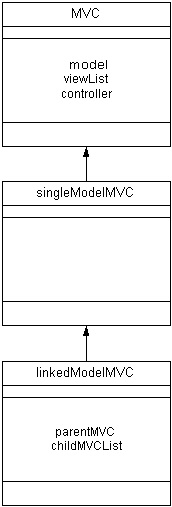
\includegraphics{fullMVCClass.jpg}}
    \caption{ The MVC class. }
    \label{Fig:MVCClass}
  \end{center}
\end{figure}

Thus, the \Rclass{linkedModelMVC} class not only binds the model,
view, and controller objects together, but it also shows
that the \Robject{linkedModelMVC} objects can be related to each other 
through a parent-child (tree) hierarchy, as shown in Figure \ref{Fig:Hier}.
In this picture, modelA is the name of the original \Robject{MVC} object
(model) and from it, two \Robject{MVC} objects were created,
modelB and modelC. Then from `modelB', three
\Robject{MVC} objects were created, modelD, modelE, and
modelF.  As an example, modelA could be gene 
expression data, modelB could be gene expression data that is a subset of
modelA (based on filtering), modelC could be derived by performing
multidimensional scaling (MDS) on modelA, modelD could be the Gene Ontology
(GO) graph representing the molecular functions of the genes in modelB,
modelE could be the KEGG pathways that the genes in modelB are involved
in, and modelF could be the chromosome locations of the genes in modelB.

\begin{figure}[ht]
  \begin{center}
    \scalebox{0.6}{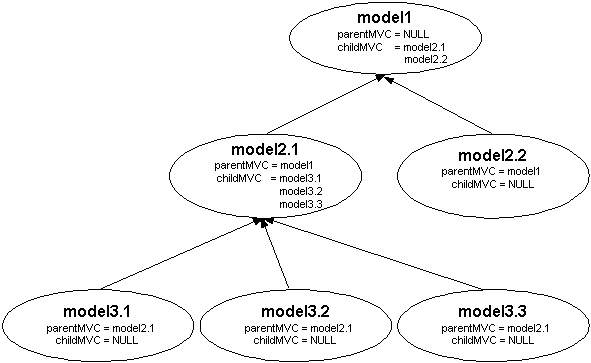
\includegraphics{Hierarchy2.jpg}}
    \caption{ The parent-child relationship between \Robject{MVCs}. }
    \label{Fig:Hier}
  \end{center}
\end{figure}

As shown in Figure \ref{Fig:Hier}, there are many cases where there are
natural submodels that can be derived from a parent model.  We propose that
each submodel is itself a \Robject{MVC} instance, and hence can have multiple
linked views.  Even though each submodel is its own \Robject{MVC} instance,
there will be times when the submodel \Robject{MVC} needs to communicate with
its parent \Robject{MVC}.  There are many different ways of communicating
between parent and child \Robject{MVCs} and we discuss this in Section
\ref{Sec:MultMVC}.

Deciding when new data should be added to the current model versus generating
a new submodel in a \Robject{MVC} instance is done by comparing the
relationship between the new data and the data in the current model.  If the
new data has a one-to-one relationship with the elements in the current model,
then we believe that in most cases the new data should be added to the 
current model.  For example, if there is
a test statistic for each row in a data frame, then this could be added to the
model.  However, if the new data has a one-to-many or a many-to-many
relationship with the elements in the current model, then serious
consideration should be given to the creation of a submodel.  If there is
already an appropriate MVC class (e.g. if the submodel is a graph) then it can
be generated by creating a new instance of the appropriate MVC class.  If there
is no appropriate implementation, then the user will need to create one.  
As an example, consider the
relationship between genes and GO terms.  If the original model contains gene
expression levels and a user wants to explore the GO terms for these genes,
then we encourage the creation of the GO graph representing the GO terms, and
creating a new graph \Robject{MVC} object.

\subsection{Messages Within a MVC Object}
\label{Ssec:OneMess}

The message classes provide communication between different
components of the MVC design, such as when the model changes a message needs
to be sent to the views to let them know that they should be updated.  This
communication between the model, view and controller is crucial for the pieces
to work together and yet, still be independent of each other.  For information
about messages that are passed between \Robject{MVC} objects, please see
Section \ref{Ssec:MultMess}. 

The object model for the message classes was derived from the idea
that all messages must have certain methods in common, such as
\Rfunction{initialize} and \Rfunction{handleMessage}, because all
messages must be created and handled in some manner so that the
message is read and acted upon.  All messages are sent to
the \Rfunction{handleMessage} method, which determines where the information
should be sent and hence, is the dispatcher.   Also, since messages
are sent when something has changed, either through addition, alteration, or
deletion, the message classes reflect only certain operations.  These
common purposes for the messages allow the message object
model to be constructed, and this model is shown in Figure \ref{Fig:Mess}.

\begin{figure}[ht]
  \begin{center}
    \scalebox{0.6}{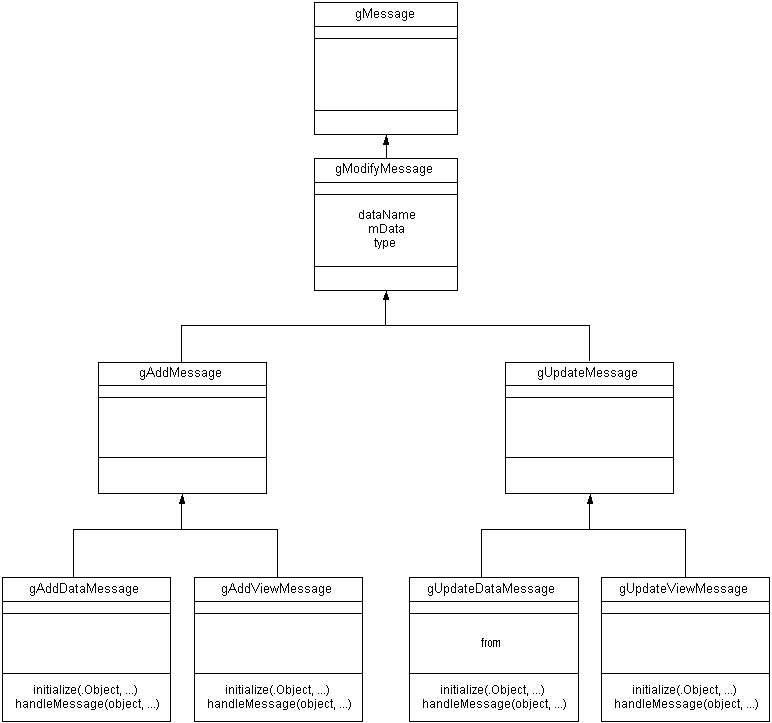
\includegraphics{newMessageClass.jpg}}
    \caption{ Inheritance for message classes. }
    \label{Fig:Mess}
  \end{center}
\end{figure}

As with the view classes, the top message class,
\Rclass{gMessage}, is a virtual class.  It contains no slots and its purpose
is to bind the other message classes together.

Currently, there are two types of messages for messaging within a
model, view, controller object: an add and an update message.  These two types
of messages are both performing some type of modification and thus, both the
add message, \Rclass{gAddMessage}, and the update message,
\Rclass{gUpdateMessage}, inherit from the virtual class,
\Rclass{gModifyMessage}, which contains three slots, \Rslot{dataName},
\Rslot{mData}, and \Rslot{type}.  \Rslot{dataName} is the character string
that gives the name of the model, \Rslot{mData} is a list of data needed to
perform the addition or alteration operation, and \Rslot{type} is a character
string that gives the type of addition or alteration to perform.  Both
\Rclass{gAddMessage} and \Rclass{gUpdateMessage} are virtual classes. 

Since adding a view requires different information and methods from adding a
model (and similarly with updating views versus models), it makes sense to
have two separate message classes for these elements.  Messages
sent between components are from one of the following classes:
\Rclass{gAddDataMessage}, \Rclass{gAddViewMessage},
\Rclass{gUpdateDataMessage}, and \Rclass{gUpdateViewMessage}.  The
\Rclass{gAddDataMessage} class represents a message to add a model
and a \Robject{MVC} object because whenever a model is added, a
\Robject{MVC} object is created that contains this model.  The
\Rclass{gAddViewMessage} class represents a message to create a view.  This
message can only be used after a model has been added. 

The \Rclass{gUpdateDataMessage} class represents a message to update
a model.  This message is crucial for linking because it is
responsible for ensuring that once a model has been updated this
information propagates to all views of the model.  This
same information must also be passed along to any other \Robject{MVC} object
that is related to this model.  Because this
information gets passed to other \Robject{MVC} objects (see Section
\ref{Sec:MultMVC}), this message also has one new slot, \Rslot{from}, in
addition to the slots it inherits from \Rclass{gUpdateMessage}.  The
\Rslot{from} slot is the name of the model that the update data
message came from.  This slot is necessary because the update data message can
come from one of two sources: the message can occur because of user
interaction with a view of this model or the message may
occur because a different model that is
linked to this model has been updated.  Thus, the update data
message may come from within this \Robject{MVC} object or it may come from
either the parent \Robject{MVC} or a child \Robject{MVC}.  Finally, the
\Rclass{gUpdateViewMessage} class represents a message to update a
view.  This message is created and handled whenever the
model is updated so that the views accurately reflect the model. 

An example of message passing within a \Robject{MVC} object is shown
in Figure~\ref{Fig:MPwithin}.  In this example, there are two views of the
model (view 1 and view 2), and the response to a user
performing a button click event over a point in the scatter plot is to
color the point red.  Setting the response to an event was discussed
in Section~\ref{Ssec:OneEvent}.  Here the user first clicks on a point
in view 1, which is shown as Step 1 (the circled 1 on the
figure).  In the figure, the point that has been clicked has an arrow
next to it.  Then, in Step 2, an update data message is sent to the
model, which updates itself accordingly, i.e. by changing the color
associated with the corresponding element.  After the model has been
updated, the views must be notified that a change has occurred so in
Step 3, an update view message is created and sent to all views of
this model.  In response to this message, the views update themselves in
Step 4 and now each view has one point that is colored red to reflect the
change in the model.

\begin{figure}[ht]
  \begin{center}
    \scalebox{0.6}{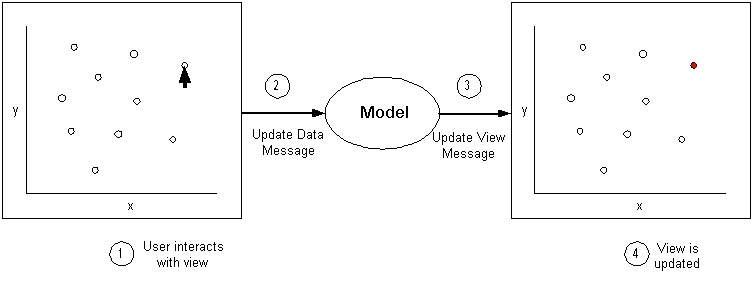
\includegraphics{newMPwithin.jpg}}
    \caption{ Message passing within a \Robject{MVC} object.  The first step,
      indicated by a circled one, occurs when a user interacts with the y
      versus x scatter plot (view 1).  Then an update data message is sent to
      the model in the second step, which alters the model.  Next in the third
      step all views of this model are sent an update view message, which
      causes the views to be updated in the fourth step. }
    \label{Fig:MPwithin}
  \end{center}
\end{figure}

All four classes, \Rclass{gAddDataMessage}, \Rclass{gAddViewMessage},
\Rclass{gUpdateDataMessage}, and \Rclass{gUpdateViewMessage}, have
\Rfunction{initialize} and \Rfunction{handleMessage} methods, which perform
the following tasks.  The \Rfunction{initialize} method is used to properly
fill the slots of the object when it is created.  The
\Rfunction{handleMessage} method is necessary to process the message.  Since a
message is a form of communication between two components, once it is created
it must be sent to the proper recipient and action must be taken in response
to its information, which is the purpose of the \Rfunction{handleMessage}
method. 

As with the inheritance structures seen in previous sections, the message
inheritance structure is designed to allow for extensibility.  For example, a
user could create a \Rclass{gUpdateControlMessage} class that inherited from
the \Rclass{gUpdateMessage} class.  This new class,
\Rclass{gUpdateControlMessage}, could convey information that told the
control window to be updated in response to a change in the active view (the
active view is the view that has the focus).  Currently, the control window
does not reflect what the active view is, but if a view was created that could
be rotated, then a user may want the control window to have some type of
interface to allow the user to control the rotation.  The goal for the message
classes is that the design is flexible enough to allow a user to make
additions or changes. 

\section{Details of Multiple MVCs}
\label{Sec:MultMVC}

We now describe the implementation of multiple \Robject{MVC} objects for
linking views of multiple linked models.  Each \Robject{MVC} object
represents one model and its views.  In our
paradigm models are linked through some additional meta-data. In
the case of gene expression data the GO view is linked to the heatmap
view through the mapping of genes to GO categories. In the city and
state example, the cities are linked via the states in which they are
contained. If, in the state MVC, a state is selected that information
can be propagated to the city MVC, but some piece of software must
link the state to the cities. 

Thinking of experimental data that are linked to meta-data as an example, there
are two \Robject{MVC} objects, one for the experimental data and one for the
meta-data.  In the example of experimental microarray data that are linked to
the Gene Ontology molecular function graph that was first mentioned in Section
\ref{Ssec:Limit}, these two models are linked in the following manner: the
Affymetrix identifiers in the experimental microarray data are linked to Locus
Link identifiers, which are in turn linked to the Gene Ontology molecular
function terms.  Thus, to pass information between these two models a table
that links Affymetrix identifiers to Gene Ontology molecular function terms
must be stored or there must be a function to call that converts from
Affymetrix identifiers to Gene Ontology molecular function terms and vice
versa.  Once it is possible to link these models, then information must be
passed between them through messages to keep the views synchronized.

As mentioned in Section \ref{Ssec:OneMVC}, the \Rclass{MVC} class has slots
for how the current \Robject{MVC} relates to other \Robject{MVC} objects and
these slots are \Rslot{parentMVC} and \Rslot{childMVCList}.  These slots show
that \Robject{MVC} objects are related through a tree hierarchy where a child
model is derived from its parent model.  
Consider Figure~\ref{Fig:Hier}, which was shown previously.  If
modelA's model changes, then this information first gets passed to
modelB and modelC and these two \Robject{MVCs} may make changes to
their models based on this information.  Then modelB passes this
information to modelD, modelE, and modelF based on the changes
that modelB made to its model.  Thus, information passing between
modelA and modelD, for instance, only occurs through modelB.  So
messages can only be sent from parent \Robject{MVC} to child
\Robject{MVC} or from child \Robject{MVC} to parent \Robject{MVC}.
This communication between parent and child \Robject{MVCs} was shown in Figures
\ref{Fig:heatmap}, \ref{Fig:GOgraph}, and \ref{Fig:heatmapsub} in Section
\ref{sec:micro}.  Here views of the parent and child models are
synchronized, but the selected items in a grandparent model may not
match the selected items in a grandchild model (as shown by Figures
\ref{Fig:heatmap} and \ref{Fig:heatmapsub} where the selected genes are
different in these two heatmaps).  Deciding how to link \Robject{MVC} models 
is a difficult task especially when the relationship between elements in the 
two models is not one-to-one.

Next we consider how the models are linked (and thus, how \Robject{MVC}
objects are linked) followed by how messages are passed between these
linked \Robject{MVC} objects. 

\subsection{Linking Models}
\label{Ssec:MultLink}

For messages to pass between \Robject{MVC} objects, the information from one
\Robject{MVC} must be converted into useful information for a different
\Robject{MVC} object.  Thus, there needs to be some way to determine how data
from one \Robject{MVC} object relates to data in a different \Robject{MVC}
object.  This conversion is done by two functions that are stored in the
\Rslot{linkData} slot of the model objects.  The \Rslot{linkData}
slot is a list with two elements: a \Rfunction{toParent} function and a
\Rfunction{fromParent} function. 

When a child \Robject{MVC} is created from an existing \Robject{MVC}, the
child model's \Rslot{linkData} slot is filled with the two functions,
\Rfunction{toParent} and \Rfunction{fromParent}.  When the model in
the child \Robject{MVC} is updated, the \Rfunction{toParent} function in the
\Rslot{linkData} slot is used to convert the child model's data
change into useful information for the parent model.  

Now suppose that the parent model changed instead.  This information
needs to be passed to the child model.  However, a parent can have
multiple child \Robject{MVC} objects so the parent sends a message to each
child \Robject{MVC} to notify the child of the change and then each child
\Robject{MVC} handles the message by using its \Rfunction{fromParent}
function.  The \Rfunction{fromParent} function converts the parent
model's data change into useful information for this
particular child model.  Thus, the message sent to all children is the
same, but each child converts the message, using its \Rfunction{fromParent}
function, to make it specific for that child.

The link functions, \Rfunction{toParent} and \Rfunction{fromParent}, can
become quite complex depending on the relationship between the elements in the
two models.  Suppose that the data elements in the two models have a
one-to-one relationship where data element 1 in child model A is linked to
data element 2 in parent model B.  Now if data element 1 in child model A is
selected, then the \Rfunction{toParent} function will pass along the
information that data element 2 in parent model B should be selected.  Here
the linking is straightforward.  However, if the data elements in the two
models have a one-to-many or many-to-many relationship, the decision about
which linked elements to update is more complex.  Now suppose that data
element 1 in child model A is linked to data elements 10, 11, and 12 in parent
model B and data element 2 in child model A is linked to data elements 12 and
13 in parent model B.  Here a many-to-many relationship exists between the
data elements.  If the user selects element 1 in child model A, the
\Rfunction{toParent} function must decide if elements 10, 11, and 12 should be
selected in parent model B or if only elements 10 and 11 should be selected in
parent model B (because element 12 in model B is also linked to element 2,
which is not selected, in model A).  

These two options for the linking function can be represented as \textit{any}
versus \textit{all} linking.  In \textit{any} linking, if any element is
updated, then the corresponding linked element is updated.  This linking could
also be represented as \textit{or} linking if one is thinking in terms of
boolean operators.  In \textit{all} linking, the element in the second model
is updated only if all linked elements are updated in the original model.
Similarly, this linking could be also be represented as \textit{and} linking
if one is thinking in terms of boolean operators.  

Making the previous example even more complex suppose that child model A also
had data element 3 which is linked to data elements 12, 13, and 14 in parent
model B.  Now if data elements 1 and 3 are selected in child model A, the
\Rfunction{toParent} function can link based on one of these options: i) select
data elements 10, 11, 12, 13, and 14 in parent model B, which indicates that
any items in model B that are linked to elements 1 and 3 in model A are
selected, ii) select data element 12, which indicates that only data elements
that are linked to both elements 1 and 3 in model A are selected, or iii)
select no data elements in model B, which indicates that only elements linked
to both elements 1 and 3 and no other elements in model A are selected.
Another consideration in the linking functions may be to change the response
depending on the type of selection being performed.  For example, \textit{any}
linking between models may be appropriate when an item in one model was
highlighted, but if an element is hidden, then \textit{all} linking may be
suitable.  This flexibility lets developers determine the appropriate
relationships between models, but also requires thoughtful responses and
potentially complex linking functions.

An example of how these functions, \Rfunction{toParent} and
\Rfunction{fromParent}, are used when messages are passed between
\Robject{MVCs} is given in Section \ref{Ssec:MultMess} where Figure
\ref{Fig:MessPass} shows the \Rfunction{toParent} function being used to
convert information from a child \Robject{MVC} object into useful information
for the parent \Robject{MVC} object.

\subsection{Messages Between MVC Objects}
\label{Ssec:MultMess}

The message classes for creating a child \Robject{MVC} from an existing
\Robject{MVC} and for sending messages between \Robject{MVC} objects are shown
in Figure \ref{Fig:BetwMess}.  The message types for passing information
between \Robject{MVCs} are similar to the messages
that are passed within \Robject{MVC} objects.  Now the add child message is
similar to the add model message, and the send parent message and the send
child message are similar to the update model message.

\begin{figure}[ht]
  \begin{center}
    \scalebox{0.6}{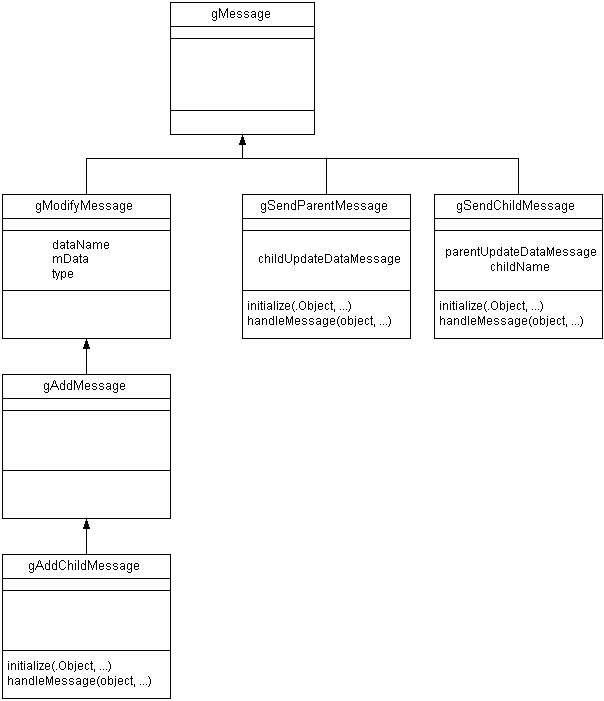
\includegraphics{MVCMessageClass2.jpg}}
%    \scalebox{0.6}{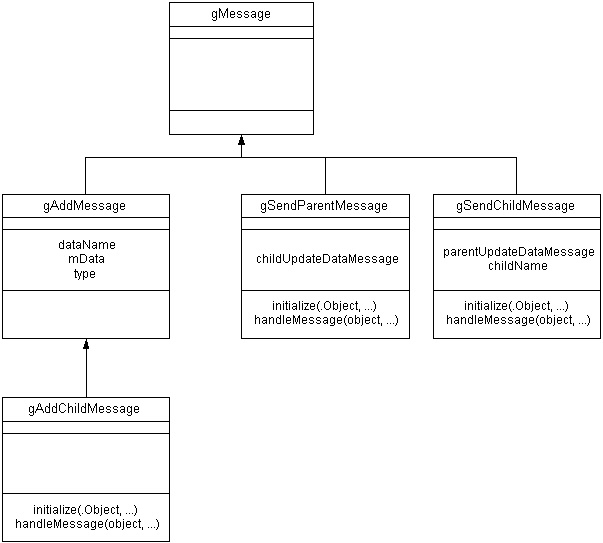
\includegraphics{newMessageClass2.jpg}}
    \caption{ Inheritance for message classes that are passed between
      \Robject{MVCs}. }
    \label{Fig:BetwMess}
  \end{center}
\end{figure}

A \Robject{gAddChildMessage} object is very 
similar to a \Robject{gAddDataMessage} object because they are both adding a
new model and a new \Robject{MVC} object.  The difference with a
\Robject{gAddChildMessage} object is that it must fill in some extra
information to tie this new \Robject{MVC} object to its parent \Robject{MVC}
object.  The \Rclass{gAddChildMessage} class inherits from the
\Rclass{gAddMessage} class, with the same slots of \Rslot{dataName},
\Rslot{mData}, and \Rslot{type}.  The \Rslot{dataName} slot is the name of the
new model (and new \Robject{MVC}), the \Rslot{mData} slot is a list that
contains the model data and virtual data to fill the \Rslot{modelData} and
\Rslot{virtualData} slots, respectively, of the new model, and the
\Rslot{type} slot gives the type of the model (currently, the options are
``exprSet'', ``graph'', or ``data.frame'').  As with the previous
message classes, the \Rclass{gAddChildMessage} class has two methods:
\Rfunction{initialize} and \Rfunction{handleMessage}.  The
\Rfunction{initialize} method properly fills the slots of the object when it
is created.  The \Rfunction{handleMessage} method ensures that the new
model and \Robject{MVC} objects are created (which is what the
\Rfunction{handleMessage} method for the \Rclass{gAddDataMessage} class does),
then it fills the \Rslot{linkData} slot of the new child model
so that the \Rfunction{toParent} and \Rfunction{fromParent} functions are
available for messaging between \Robject{MVC} objects, and finally it stores
information in the child \Robject{MVC} object's controller that determines if
the child model was created from a subset of the parent
model.  Thus, the \Rfunction{handleMessage} method for the
\Rclass{gAddChildMessage} class both creates the child \Robject{MVC} object
and relates it to the parent \Robject{MVC} object. 

The next two message classes pertain to sending information to linked
\Robject{MVC} objects when a parent \Robject{MVC} or child \Robject{MVC}
object has changed.  These classes are \Rclass{gSendParentMessage} and
\Rclass{gSendChildMessage} and they both inherit from the \Rclass{gMessage}
class, as shown in Figure \ref{Fig:BetwMess}.  Because the messages are
sending information to a linked \Robject{MVC} object, they both contain a slot
for a \Robject{gUpdateDataMessage} object that was just used to update a
\Robject{MVC} object.  The \Rclass{gSendParentMessage} class has one slot,
\Rslot{childUpdateDataMessage}, and this slot contains the
\Robject{gUpdateDataMessage} object that was used to update the child
model.  Similarly, the \Rclass{gSendChildMessage} class has two
slots, \Rslot{parentUpdateDataMessage} and \Rslot{childName}, where the
\Rslot{parentUpdateDataMessage} slot contains the \Robject{gUpdateDataMessage}
object that was used to update the parent model and the
\Rslot{childName} slot contains the name of the child model that is
being updated because a parent \Robject{MVC} can have more than one child
\Robject{MVC}.  

As with all the other message classes, these two send messages have
two methods: \Rfunction{initialize} and \Rfunction{handleMessage}.  The
\Rfunction{initialize} method properly sets the slots of the new object.  The
\Rfunction{handleMessage} method for a \Robject{gSendParentMessage}
takes the \Robject{gUpdateDataMessage} object from the child model
and converts it to a \Robject{gUpdateDataMessage} object for the parent
model using the \Rfunction{toParent} function.  Similarly, the
\Rfunction{handleMessage} method for a \Robject{gSendChildMessage} takes the
\Robject{gUpdateDataMessage} object from the parent model and
converts it to a \Robject{gUpdateDataMessage} object for the child
model using the \Rfunction{fromParent} function.  An example of how
these messages are passed and converted is shown in Figure \ref{Fig:MessPass}.

These message classes ensure that when a model is updated, its parent and
child models are notified of the change and most importantly, are
notified of the change in a way that each model can properly act upon that
information.  Because each \Robject{MVC} object has a different model (and
thus a different data set and potentially a different data structure),
information that pertains to the model for one \Robject{MVC} must be converted
to useful information for the linked model and this conversion is done by the
\Rfunction{toParent} and \Rfunction{fromParent} functions.  

\begin{figure}[ht]
  \begin{center}
    \scalebox{0.55}{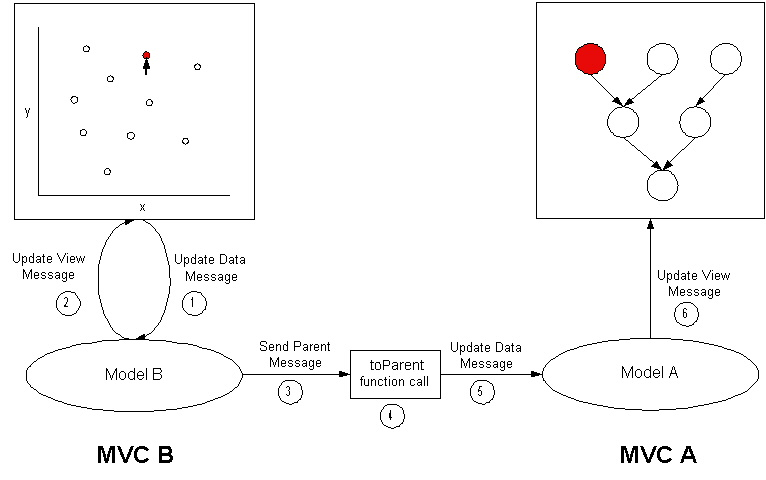
\includegraphics{newMP.jpg}}
    \caption{ Message passing between and within \Robject{MVCs}.  When a user
      interacts with the y versus x scatter plot, the first step, indicated by
      a circled one, is to send an update data message to model B.  After
      model B has been updated, all views of this model must be notified, which
      is shown in the second step when an update view message is sent.  Next
      any data that are linked to model B must be notified that model B
      changed, which is shown in the third step as a send parent message.
      This message is converted into useful information for model A in
      the fourth step by the \Rfunction{toParent} function, and this
      information is sent to model A in the fifth step when an update data
      message is sent.  Finally, after model A is updated, an update view
      message is sent in the sixth step to update all views of model A. }
    \label{Fig:MessPass}
  \end{center}
\end{figure}

Figure \ref{Fig:MessPass} is very similar to Figure \ref{Fig:firstMP} shown in
Section \ref{Sec:Methods}.  Now, however, Figure \ref{Fig:MessPass} shows how
\Robject{MVC} objects are defined and how messages are passed within one
\Robject{MVC} as well as how this information gets passed on to its parent
\Robject{MVC} using messages.  Suppose for this example that when the user
clicks a mouse button over the scatter plot, the response to this event is to
color the point under the cursor 
red.  In this picture, the message passing starts when a user clicks a point,
that is indicated by the arrow, on the scatter plot.  An update data message is
sent to Model B in response to this user interaction.  As soon as Model B is
updated, it sends an update view message to all its views so that the views
are updated to reflect the changed data.  Now the scatter plot point that was
initially clicked is red.  Then a send parent message is sent because MVC
B, which is the \Robject{MVC} object for Model B, has a parent \Robject{MVC},
which is MVC A.  Next the \Rfunction{toParent} function converts the child's
update data message into an update data message that the parent \Robject{MVC}
understands.  Then the update data message that was created by the
\Rfunction{toParent} function is sent to Model A.  Finally, after Model A has
been updated, an update view message is sent to all of Model A's views.  It is
in this last step that the view of Model A has a point colored red to indicate
which data from Model A are linked to data from Model B.  All of the data and
the views are synchronized. 

\section{Conclusions}
\label{Sec:Conc}

The goals for this research were to create software implementations and
conceptual paradigms to support the use of linked views of linked data sets,
to create interactive views where the response to an event can be changed, and
to create an extensible design that allows future users to make additions.
The first goal was accomplished by implementing \Robject{MVC} objects as
components that communicate with each other through messages.  Encapsulating
each data set in a \Robject{MVC} object was particularly useful because it
allowed the reuse of code for communicating between the components of a
\Robject{MVC} object, which made generating new model and view classes easier.
However, communication between the \Robject{MVC} objects was, at times, more
complicated. 

The crux of the communication between \Robject{MVC} objects is the link
function, which converts information that one model can understand into
information that a linked model can understand.  As discussed previously, the
linking functions, \Rfunction{toParent} and \Rfunction{fromParent}, can be
quite complex if the relationship between the data elements in the two models
is one-to-many or many-to-many.  In response to an update in one model, the
linking function must decide if all linked elements in the second model
should be updated, if any linked elements should be updated, or if a subset of
linked elements should be updated.  These decisions must be made by the
developer to properly represent the relationship between the data elements in
the two models.  While this flexibility lets the developer represent different
relationships between different models, the developer is then responsible for
knowing what makes sense (for example, biologically) when creating the link
functions. 

The second goal of creating interactive views was met by using the
\Rpackage{RGtk} and \Rpackage{gtkDevice} packages to create devices that could
respond to events.  Using these packages made creating interactive views
particularly straightforward because any static R plot could be made
interactive by plotting it on a Gtk device and by having the plotting function
return information about the location of plot objects on the device.  In
addition the \Rclass{gEventFun} class was designed so that users could alter
the response to an event.  The response to an event could be as simple as
selecting the plot object that was just clicked by a mouse button or the
response could be as complicated as creating a new model.  This flexibility
lets the developer create a more varied interactive environment.

Finally, the last goal of creating an extensible design was achieved through
the inheritance structure for classes, which allows for extensions by the
user, and through command line functions, which let the user create new menu
items to add to the GUI and also let the user create new callback functions
that can be linked to events.  However, in terms of extensibility, certain
design decisions, such as expecting the models to be linked through a
parent-child hierarchy, may not work with some models.  As an example, the
linked tables from a relational database are not related through a tree
structure and thus, having parent and child \Robject{MVC} objects may not make
sense with these models.  However, the design allows users to add new types
of models, new types of views, and new message classes so there is still
flexibility for additions as long as the models are connected through
parent-child relationships.  These new class definitions could be created by
the user in a new package that extends the \Rpackage{MVCClass} package that
was discussed in this paper.  Other additions that the user may want to
perform, such as adding new menus to the GUI and adding new responses to an
event can be performed through command line functions that are defined in the
\Rpackage{iSNetwork} package, which is the front end for the design
described in this paper. 

The functionality that is provided in the \Rpackage{iSNetwork} package, which
is an implementation of the research discussed in this paper, is
discussed in detail in the vignette for this R package.  Users can load data,
create views of the data, interact with these views and change the response to
the interaction (these interactions include mouse button click events and
mouse movement events), and users can create child \Robject{MVC} objects
through the GUI or through command line functions.  With the functionality in
the \Rpackage{iSNetwork} package, the user can create views of linked models
and can explore visually the relationships between variables in different data
sets.  This functionality was implemented by extending the MVC paradigm in a
very natural way to encompass a much richer class of models and user
interactions. 

\section*{Acknowledgements}
We are indebted to Dr. Duncan Temple Lang for the creation of the
\Rpackage{RGtk} and \Rpackage{gtkDevice} packages as well as helpful advice on
their use.  

\bibliography{paper2}

\end{document}